\subsection{UC14 - Visualizzazione Ore Consuntivate }
\begin{itemize}
	\item \textbf{Identificativo}: UC14
	\item \textbf{Nome}: Visualizzazione Ore Consuntivate
	\item\textbf{Descrizione Grafica}: 
	\begin{center}
		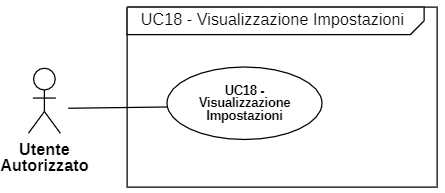
\includegraphics[scale=0.65]{images/UC14.png} 
	\end{center}

	\item \textbf{Attori}
	\begin{itemize} 
		\item \textit{Primari}: Utente autorizzato
		\item \textit{Secondari}: Non presenti
	\end{itemize}
	\item \textbf{Descrizione}: l'utente richiede di visualizzare le ore consuntivate; vengono restituite e mostrate tramite chatbot.
	\item \textbf{Precondizione}: Utente ha effettuato il login e si trova nella chat.
	\item \textbf{Postcondizione}: Chatbot restituisce la lista delle Ore consuntivate
	\item \textbf{Scenario principale}:  
		\begin{enumerate}
			\item Utente invia un messaggio al chatbot : "Quante ore ho consuntivato oggi?";
			\item Chatbot restituisce la lista delle Ore consuntivate, con eventuali informazioni.
		\end{enumerate}
\end{itemize}